\documentclass[11pt]{article}
\usepackage[english]{babel}
%\usepackage{fancyhdr, blindtext}
%\usepackage{lastpage}
\usepackage{graphicx}

\def\mytitle{Linear Elasticity}
\def\myauthor{Borek Patzak}
\def\mydate{11/09/2019}

\usepackage{fancyhdr, blindtext}
\usepackage{lastpage}

\pagestyle{fancyplain}

\fancyhead{}
\fancyfoot{}
\fancyhead[L]{\bf \mytitle}
\fancyhead[R]{\large OOFEM.ORG}
\fancyfoot[L]{Responsible: \myauthor}
\fancyfoot[R]{Date: \mydate\ Page:\ \thepage/\pageref{LastPage} }
\renewcommand{\headrulewidth}{0.4pt}
\renewcommand{\footrulewidth}{0.4pt}
\setlength\headheight{14pt}

\fancypagestyle{titlestyle}{%
    \fancyhead[L]{}
    \fancyhead[R]{\large OOFEM.ORG}
    \lfoot{Responsible:~\myauthor}
    \renewcommand{\headrulewidth}{0.4pt}
    \renewcommand{\footrulewidth}{0.4pt}
}
 
%Redefine chapter by adding special first chapter page page-style
%\makeatletter
%    \let\stdchapter\chapter
%    \renewcommand*\chapter{%
%    \@ifstar{\starchapter}{\@dblarg\nostarchapter}}
%   \newcommand*\starchapter[1]{\stdchapter*{#1}\thispagestyle{chapterstyle}}
%    \def\nostarchapter[#1]#2{\stdchapter[{#1}]{#2}\thispagestyle{chapterstyle}}
%\makeatother

\renewcommand{\maketitle}[1]{
    %\begin{titlepage}
        %{
        \thispagestyle{titlestyle}
        \vspace*{15em}
        \noindent{\Huge \mytitle}\\
        \noindent\rule{\textwidth}{0.4pt}\\[2em]
        {\bf Summary}\\[0.5em]
        #1
        \newpage
        %}
    %\end{titlepage}
}


\newcommand{\mbf}[1]{\mbox{\boldmath$#1$}}
\font\mbff=cmbsy10\def\mbfx#1{\hbox{\mbff#1}}%\let\mbf\Mbff
\newcommand{\del}[2]{\mbox{$\displaystyle\frac{#1}{#2}$}}
\newcommand{\pard}[2]{\del{\partial \,{#1}}{\partial \,{#2}}}
\newcommand{\ppd}[2]{\del{\partial \,{#1}}{\partial \,{#2}}}
\newcommand{\dpd}[2]{\del{\partial ^{2}\,{#1}}{\partial \,{#2}^{2}}}
\newcommand{\tpd}[2]{\del{\partial ^{3}\,{#1}}{\partial \,{#2}^{3}}}
\newcommand{\cpd}[2]{\del{\partial ^{4}\,{#1}}{\partial \,{#2}^{4}}}
%\newcommand{\spd}[1]{\del{\partial ^{3}\,{#1}}{\partial \,x\,\partial \,t^{2}}}
%\newcommand{\scpd}[1]{\del{\partial ^{4}\,{#1}}{\partial \,x^{2}\,\partial
%\,t^{2}}}
\newcommand{\der}[2]{\del{d \,{#1}}{d \,{#2}}}
\newcommand{\dd}[2]{\del{d ^2\,{#1}}{d \,{#2}^2}}
\newcommand{\td}[2]{\del{d ^3\,{#1}}{d \,{#2}^3}}
\newcommand{\cd}[2]{\del{d ^4\,{#1}}{d \,{#2}^4}}
\newcommand{\MKP}{{MKP$\;\;$}}
\newcommand{\inl}[2]{\mbox{$\displaystyle\int_{#1}^{#2}$}}
\newcommand{\sul}[2]{\mbox{$\displaystyle\sum_{#1}^{#2}\,$}}
\newcommand{\limit}[1]{\mbox{$\displaystyle\lim_{#1}$}}
\newcommand{\vp}{\varphi}
\newcommand{\e}{\mbf{\varepsilon}}
\newcommand{\ep}[0]{\mbf{\varepsilon}^p}
\newcommand{\epd}[0]{\dot{\mbf{\varepsilon}}^p}
\newcommand{\sig}{\mbf{\sigma}}
\newcommand{\sigs}{\sigma}%scalar
\newcommand{\kap}{\mbf{\kappa}}

\newcommand{\vsigrate}{\dot {\mbf{\sigma}}}
\newcommand{\sigrate}{\dot {\sigma}}
\newcommand{\taurate}{\dot {\tau}}
\newcommand{\erate}  {\dot {\mbf{e}}}

\newcommand{\rest}[1]{\Re\left( {#1} \right)}
\newcommand{\refeq}[1]{Eq.~(\ref{#1})}
\newcommand{\reffig}[1]{Fig.~(\ref{#1})}
\newcommand{\refeqs}[2]{Eqs.~(\ref{#1}), (\ref{#2})}
\newcommand{\refeqsr}[2]{\mbox{Eqs.~(\ref{#1})-(\ref{#2})}}

\newcommand{\C}{$^{\circ}\mathrm{C}$}
\newcommand{\ymu}{y_{\mu}}
\newcommand{\y}[1]{y_{#1}}
\newcommand{\ymui}[1]{y_{\mu_{#1}}}
\newcommand{\tdymu}{{\dot y}_{\mu}}
\newcommand{\ttdymu}{{\ddot y}_{\mu}}
\newcommand{\timeder}[1]{\dot {#1}} 
\newcommand{\dprime}{\prime\prime}

\newcommand{\beq}{\begin{equation}}
\newcommand{\eeq}{\end{equation}}
\newcommand{\bea}{\begin{eqnarray}}
\newcommand{\eea}{\end{eqnarray}}
\newcommand{\vsi}{\mbf{\sigma}}
\newcommand{\vep}{\mbf{\varepsilon}}
\newcommand{\eps}{\varepsilon}
\newcommand{\mD}{\mbf{D}}
\newcommand{\vxi}{\mbf{\xi}}
\newcommand{\vx}{\mbf{x}}
\newcommand{\dxi}{\;\mbox{d}\mbf{\xi}}
\newcommand{\vf}{\mbf{f}}
\newcommand{\vg}{\mbf{g}}
\newcommand{\veps}{\mbf{\varepsilon}}
\newcommand{\mB}{\mbf{B}}
\newcommand{\vsig}{\mbf{\sigma}}
\newcommand{\vd}{\mbf{d}}
\newcommand{\mK}{\mbf{K}}
\newcommand{\macbra}[1]{\langle{#1}\rangle}
\newcommand{\vbs}{\mbf{b}^{\sigma}}
\newcommand{\vbe}{\mbf{b}^{\eta}}
\newcommand{\vbeT}{\mbf{b}^{\eta T}}

\newcommand{\ud}{\mathrm{d}}
\newcommand{\grad}{\nabla}
%position vectors
\newcommand{\x}{\mbf{x}}
\newcommand{\xd}{\mbf{x}^\varphi}
%displacement
\newcommand{\du}{\mbf{u}} 
\newcommand{\bestresultcolor}{blue}
\newcommand{\bestresult}[1]{\textcolor{\bestresultcolor}{\bf{#1}}}
\newcommand{\ignore}[1]{}





\newcommand{\oofem}{\htmladdnormallink{OOFEM}{http://www.oofem.org}\ }
\newcommand{\oofemlnk}[1]{\htmladdnormallink{#1}{http://www.oofem.org}\ }
\newcommand{\bp}{\htmladdnormallink{Bo\v{r}ek Patz\'{a}k}{http://mech.fsv.cvut.cz/~bp/bp.html}}



\begin{document}
\maketitle{This document contains introduction to linear elasticity.}
% Basic equations
\section{Linear elasticity}
\subsection{Linear kinematics}
Let us consider a deformable body as a collection of points, where position of each point is denoted as $\x\in\Omega$. In a deformed configuration the position of each point is identified by its position vector $\xd(x) = \mbf{\phi}(\x)$. The displacement vector is then defined as:
\begin{equation}
  \label{eq:displacementvector}
  \xd(\x) = \x + \du(\x)  
\end{equation}

Let us now examine the position in a local neighborhood of a point. The deformed position of such neighbor point with coordinates $\x+d\x$ (where d\x is infinitisemally small vector) is
$$\xd(\x+d\x) = \x+d\x+\du(\x+d\x) = \xd + d\xd$$,
where $d\xd$ is the mapping of vector $d\x$ onto deformed configuration, see Fig.~\ref{fig:deformedconfiguration}.
\begin{figure}
  \begin{center}
    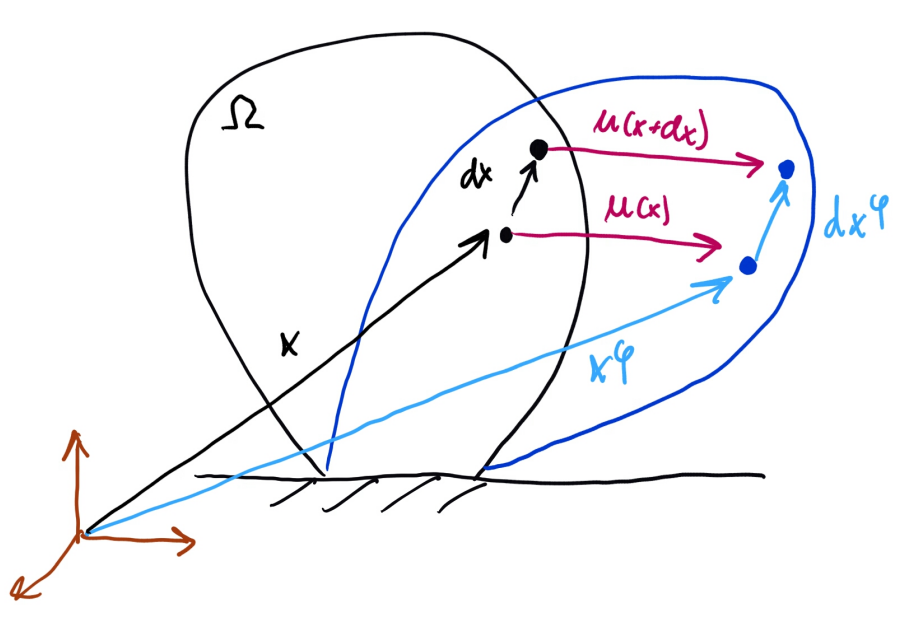
\includegraphics[width=0.5\textwidth]{deformedconfiguration.png}
  \end{center}
  \label{fig:deformedconfiguration}
  \caption{Deformed configuration}
\end{figure}
Taking into account the definition of displacement vector ~\ref{eq:displacementvector} and using Taylor formula we get
\begin{equation}
  d\xd = \x+d\x+\du(\x+d\x)-\xd = d\x-\du(\x)+\du(\x+d\x) \approx [\mbf{I}+\grad\du(\x)]d\x
\end{equation}
where $\grad\du(\x)$ is the displacement gradient tensor (in small strain theory we assume $\vert\vert\grad\du(\x)\vert\vert \ll 1$).
The displacement gradient tensor can be decomposed into symetric and antisymmetric parts
$$
\grad\du = \mbf{\eps}+\mbf{\omega}={1\over 2}(\grad\du+\grad\du^T)+{1\over 2}(\grad\du-\grad\du^T) = \grad^s\mbf{u}+\grad^a\mbf{u}
$$

The antisymmetric part corresponds to infinitesimal rotation. The symmeric part of displacement gradient tensor is therefore the measure of infinitesimal deformation
$$
d\xd = \mbf{\eps} d\x
$$
\subsection{Equlibrium equations}
Stress is defined as the force across a "small" boundary per unit area of that boundary, for all orientations of the boundary. In the most general case, called triaxial stress, the stress is nonzero across every surface element. Cauchy observed that the stress vector $\mbf{t}$ across a surface is a linear function of the surface's normal vector $\mbf{n}$:
$$
\mbf{t}(x)=\mbf{\sigma}(x)\mbf{n}(x)
$$
where $\mbf{\sigma}(x)$ is called the (Cauchy) stress tensor, completely describing the stress state at any point.
\begin{figure}
  \begin{center}
    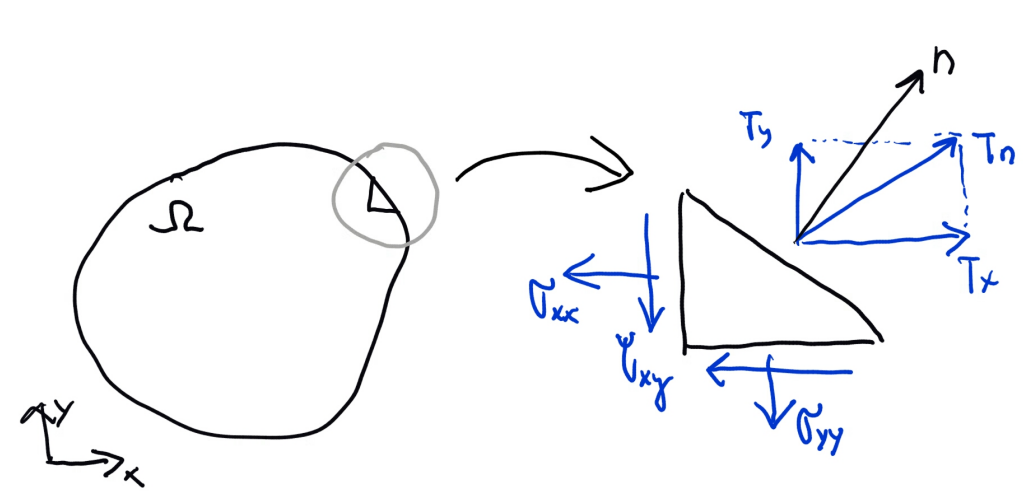
\includegraphics[width=0.5\textwidth]{tractionstressrelation.png}
  \end{center}
  \label{fig:tractionstressrelation}
  \caption{Balance between tractions and stresses in 2D}
\end{figure}

The components of the Cauchy stress tensor at every point in a material satisfy the equilibrium equations (Cauchy’s equlibrium equations). From the conservation of angular momentum follows the symmetry of the stress tensor. Therefore, the stress state of the medium at any point and instant can be specified by only six independent parameters, rather than nine. These may be written
$$
\left[
  \begin{array}{ccc}
    \sigma_{xx} & \tau_{xy} & \tau_{xz}\\
    \tau_{xy} & \sigma_{yy} & \tau_{yz}\\
    \tau_{zx} & \tau_{zy} & \sigma_{zz}
  \end{array}
\right] 
$$
where the elements $\sigma_{xx}, \sigma_{yy}, \sigma_{zz}$ are called the normal stresses (relative to the chosen coordinate system), and $\tau_{yz}, \tau_{xz}, \tau_{xy}$ the shear stresses.

In a static equlibrium, the Cauchy stress components in every material point satisfy the equilibrium equations, see~ref{fig:stressbalance}
\begin{equation}
  \sigma_{ji, j} + F_i = 0
\end{equation}
where we use summation convention over repated indices and $F_i$ are the components of the body force. In a compact tensorial notation we can write the above equation as
\begin{equation}
  \grad\cdot\sigma + F_i = 0
  \label{eq:staticequlibrium3d}
\end{equation}

\begin{figure}
  \begin{center}
    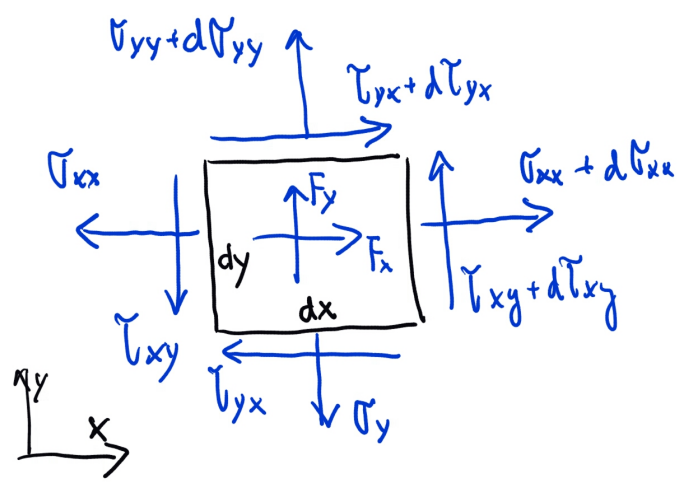
\includegraphics[width=0.5\textwidth]{stressbalance2d.png}
  \end{center}
  \label{fig:stressbalance}
  \caption{Stress balance in 2D}
\end{figure}

\subsection{Constitutive equations}
In this section we present the constituve relations (i.e. relations between stress and strain tensors) for the case of hyperelasticity, which could be defined in terms of strain energy density $W(\mbf{\eps})$, which allows to evaluate stress components as partial derivatives:
$$
\sigma_{ij}=\pard{W}{\eps_{ij}}
$$
For example, the Hooke's law  is defined using following strain energy potential
$$
W(\eps) = \del{1}{2}\eps_{ij}\mbf{C}_{ijkl}\eps_{kl}
$$
where $\mbf{C}$ is forth order elasticity tensor. The equality of mixed derivatives $(\dpd{W}{\eps_{ij}\eps_{kl}} = \dpd{W}{\eps{kl}\eps{ij}})$ and symmetry of stress and strain tensors $\pard{\sigma{ij}}{\eps_{kl}} = C_{ijkl}=C_{jikl}=C_{ijlk}$ imply that there is in general maximum 21 independ components of the elasticity tensor.
In the simplest case, the elasticity tensor for isotropic linear elastic material  can be described by only two parameters: either Lame\'s parameters ($\lambda, \mu$) or more usual parametrs being Young's modulus $E$ and Poisson's ratio $\nu$:
$$
C_{ijkl}=\lambda\delta_{ij}\delta_{kl}+2\mu {1\over 2}[\delta_{ik}\delta_{jl}+
 \delta_{il}\delta_{jk}] \equiv \mbf{C}=\lambda\mbf{1}\otimes\mbf{I}+2\mu\mbf{I}
$$

\subsection{Voight notation}

The Voigt notation is hrequantly used to take advantage of the symmetry of the stress tensor to express the stress tensor as a six-dimensional vector of the following form:
$$
\tilde{\mbf{\sigma}}=
\left[
  \sigma_{x}, \sigma_y, \sigma_z, \tau_{yz}, \tau_{xz}, \tau_{xy}
  \right]^T \equiv
\left[
  \sigma_{xx}, \sigma_{yy}, \sigma_{zz}, \tau_{yz}, \tau_{xz}, \tau_{xy}
  \right]^T
$$

The strain tensor, similar in nature to the stress tensor (both symmetric second-order tensors) can be written in Voight notation as
$$
\tilde{\mbf{\eps }}=
\left[
  \eps_{x}, \eps_y, \eps_z, \gamma_{yz}, \gamma_{xz}, \gamma_{xy}
  \right]^T \equiv
\left[
  \eps_{xx}, \eps_{yy}, \eps_{zz}, 2\eps_{yz}, 2\eps_{xz}, 2\eps_{xy}
  \right]^T
$$

The benefit of using different representations for stress and strain is the scalar invariance
$$
\mbf{\sigma}\cdot\mbf{\eps}=\sigma_{ij}\eps_{ij}=\tilde{\sigma} \tilde{\eps}
$$
Similarly, a three-dimensional symmetric fourth-order tensor can be reduced to a [6,6] matrix.


\subsection {Boundary value problem in small strain elasticity}
\subsubsection{Strong form}

Starting from the equilibrium equations~ref{eq:staticequlibrium3d}, into which we can substitute the constituve equations and strain-displacement relation we obtain the equlibrium equation expressed in terms of displacements:
$$
\pard{}{x_j}\left({C_{ijkl} {1\over 2}(\pard{u_k}{x_l}+\pard{u_l}{x_k})}\right) + F_i = 0
$$
This system of three partial differnetial equations can be solved, provided that appropriate boundary conditions are given. In summary, the strong form is the following:\\
\begin{center}
\fbox{
  \begin{minipage}{8cm}
    Find $\mbf{u}\in R^n$, such that\\[4mm]
    $\pard{}{x_j}\left({C_{ijkl} {1\over 2}(\pard{u_k}{x_l}+\pard{u_l}{x_k})}\right) + F_i = 0 \in \Omega\,$\\[2mm]
    $\mbf{u}=\mbf{\bar{u}} \in \Gamma_u$\\[2mm]
    $\mbf{t}^n_i = C_{ijkl}{1\over 2}(\pard{u_k}{x_l}+\pard{u_l}{x_k})\,n_j = \bar t_i \,\in \Gamma_t$
  \end{minipage}
}
\end{center}

\subsubsection{Weak form}

  By following the method of weighted residuals, we multiply the governing differential equations~\ref{eq:staticequlibrium3d} in residual form by a sutable test functions $\delta\mbf{u}$, satisfying the homogeneous boundary conditions on $\Gamma_u$
  $$
  \int_\Omega \delta\mbf{u} \cdot \left(
  \grad\cdot\mbf{\sigma} + F \right)\ d\Omega = \mbf{0}
  $$
  By applying the Green's formula, we arrive at
  $$
  \int_\Omega\grad\delta\mbf{u}\cdot\mbf{\sigma}\ d\Omega =
  \int_\Omega\delta\mbf{u}\cdot\mbf{F}\ d\Omega + \int_\Gamma\delta\mbf{u}\cdot\mbf{\sigma}\mbf{n}\ d\Gamma
  $$
  Then we can substitute for the stresses and tractions and taking into account the symmetry of stress tensor ($\sigma=C\mbf{\eps})$
  \begin{equation}
  \int_\Omega\grad^s\delta\mbf{u}\cdot\mbf{C}\mbf{\eps}\ d\Omega =
  \int_\Omega\delta\mbf{u}\cdot\mbf{F}\ d\Omega + \int_\Gamma\delta\mbf{u}\cdot\mbf{t}\ d\Gamma
  \label{weakform3d}
  \end{equation}
  Or, equaivalently using Voight's notation
  \begin{equation}
  \int_\Omega\delta\tilde{\eps}^T\tilde{\mbf{D}}\tilde{\mbf{\eps}}\ d\Omega =
  \int_\Omega\delta\mbf{u}^T\mbf{F}\ d\Omega + \int_\Gamma\delta\mbf{u}^T\mbf{t}\ d\Gamma
  \label{eq:weakformvoight}
  \end{equation}
  
  Note: this is equaivalent to the principle of virtual displacements. For hyperelastic material, the weak form is identical to the principle of minimum potential energy.

  
\subsection{Finite element discretization}
Let us consider discretization of the problem domain $\Omega$ into set of nonoverlapping subdomains $\Omega_e$, called elements.
Next we will consider the approximation of the unknown displacement field, defined on individual subdomains. Note that the approximation is not arbitrary:
\begin{itemize}
  \item The weak form kontains only first derivatives of the unknown and test functions, thus only $C^0$ continuity is required.
\end{itemize}
The element approxiamtion of the arbitrary function $f$ has the form
$$
f = \sum N_j(\mbf{x})r_j  = \mbf{N}\mbf{r}
$$
where $N_j$ are so called shape or approximation functions and $r_j$ are nodal values.
Note that for the approximation functions to be interpolatory, the shape functions have to satisfy Kronecker-delta property, i.e., $N_j(\mbf{x}_i)=\delta_{ij}$, where $\mbf{x}_i$ is the position vector of the i-th node. Also, the shape functions have to satisfy the condition $\sum N_i=1$, which follows from the requirement to approximate the constant function.
The required continuity of element approximations have to be satisfied. This is typically achieved by enforcing the continuity at the nodal points.
In our case, the approximation of displacements and test functions is
\begin{eqnarray}
  \mbf{u}^e&=&\mbf{N}^e(\mbf{x})\mbf{r}^e\\
  \delta\mbf{u}^t&=&\mbf{N}^e(\mbf{x})\delta\mbf{r}^e
\end{eqnarray}

We will use the weak form~\ref{weakform3d}, which using Voight's notation has the form
$$
  \int_\Omega\grad^s\delta\mbf{u}\cdot\mbf{C}\mbf{\eps}\ d\Omega =
  \int_\Omega\delta\mbf{u}\cdot\mbf{F}\ d\Omega + \int_\Gamma\delta\mbf{u}\cdot\mbf{t}\ d\Gamma
$$

  We will need also the derivatives of the displacement and test functions
  \begin{eqnarray}
  \tilde{\eps}^e = = \mbf{B}^e(\mbf{x})\mbf{r}^e\\
  \delta\tilde{\eps}^e&=&\mbf{B}^e(\mbf{x})\delta\mbf{r}^e
\end{eqnarray}
where $B^e$ matrix contains the first partial derivatives of the shape functions. 
By substiituting into the weak form~\ref{eq:weakformvoight} we obtain
\begin{equation}
  \sum_e \delta\mbf{r}^{e,T}
  \left[
    \underbrace{\int_{\Omega^e} \mbf{B}^{e,T}\tilde{\mbf{D}}^e\mbf{B}^e\mbf{r}^e\ d\Omega}_{\mbf{K}^e}\mbf{r}^e-\underbrace{\int_{\Omega}\mbf{N}^{e,T}\mbf{F}\ d\Omega}_{\mbf{f}^e_\Omega} - \underbrace{\int_{\Gamma_t}\mbf{N}^{e,T}\bar{\mbf{t}}\ d\Gamma}_{\mbf{f}^e_\Gamma}
    \right] = \mbf{0}
\end{equation}

After introducing a mappig between element displacement vectors $\mbf{r}^e$, nodal vectors of test function values $\delta\mbf{r}$ and their global counterparts $\hat{\mbf{r}}, \delta\hat{\mbf{r}}$ one can obtain
\begin{equation}
  \delta\hat{\mbf{r}}^{T}
  \left[
    \hat{\mbf{K}}\hat{\mbf{r}}-\hat{\mbf{f}}_\Omega - \hat{\mbf{f}}_{\Gamma}
    \right] = \mbf{0}
\end{equation}
By taking into account that the test fuctions are arbitrary (i.e. $\delta\hat{\mbf{r}}\ne\mbf{0}$), one finnaly obtains the following set of linear algebraic equations for unknonwn nodal displacements $\hat{\mbf{r}}$:
\begin{equation}
    \hat{\mbf{K}}\hat{\mbf{r}}=\hat{\mbf{f}}_\Omega + \hat{\mbf{f}}_{\Gamma}
\end{equation}

\section{Implementation}
The linear elasticity is implemented by {\em LinearStatic} and {\em StaticStructural} engineering models. The {\em LinearStatic} model supports multiple load cases, as the load vector is formed for each dicrete time step representing the load case. By default, the ith load case corresponds to time step at time i. 
\end{document}